\documentclass[10pt, journal, compsoc]{IEEEtran}
\usepackage{colortbl}
\usepackage{booktabs}
\usepackage{subcaption}
\usepackage{algorithm}
\usepackage{algorithmicx}
\usepackage{algpseudocode}
\usepackage{tabulary}
\usepackage{bigstrut}
\usepackage{graphicx}
\linespread{1}
\setlength\fboxsep{1pt}
\setlength\fboxrule{1pt}
\usepackage{multicol}
\bstctlcite{IEEEexample:BSTcontrol}
\usepackage[table]{xcolor}
\usepackage{picture}
\newcommand{\quart}[4]{\begin{picture}(100,3)
{\color{black}\put(#3,3){\circle*{4}}\put(#1,3){\line(1,0){#2}}}\end{picture}}
\usepackage{amsmath}
\usepackage{balance}
\usepackage{flushend}
\usepackage[english]{babel}
\usepackage{blindtext}
\usepackage{times}
\usepackage{cite}
\usepackage{hyperref}
\hypersetup{
  colorlinks = false,
  hidelinks = true
}
\newcommand{\bi}{\begin{itemize}}
  \newcommand{\ei}{\end{itemize}}
\newcommand{\be}{\begin{enumerate}}
  \newcommand{\ee}{\end{enumerate}}
\newcommand{\tion}[1]{\textsection\ref{sec:#1}}
\newcommand{\fig}[1]{Figure~\ref{fig:#1}}
\setlength{\parindent}{0em}
\setlength{\parskip}{1em}


\begin{document}
  \markboth{CSC 712: Software Testing and Reliability. Fall, 
    2014}%
  {CSC 712 Software Testing and Reliability. Fall, 
    2014}
  
  \title{On Strategies for Improving Software Defect Prediction}
  \author{Rahul Krishna, 
    \IEEEauthorblockA{\normalsize {\textit{Dept. of Electrical and Computer 
          Engineering}\\
        North Carolina State University, Email: 
        \href{mailto:rkrish11@ncsu.edu}{{rkrish11@ncsu.edu}}}}}
  
  \IEEEcompsoctitleabstractindextext{%
    \begin{abstract}
      Programming inherently introduces defects into programs, as a result software systems can crash or fail to deliver an important functionality. It is very important to test a software throughly before it can be used. But an extensive testing can be prohibitively expensive or may take too much time to conduct This necessitates the use of automated software defect prediction tools. Although numerous machine learning algorithms are available to detect defects in software, but several factors undermine the accuracy of such algorithm. This paper uses Classification and Regression Trees (CART) and Random Forests to examines two approaches to counter the aforementioned problem. The first approach involves the use Synthetic Minority Oversampling Technique (also known as SMOTE). The second approach attempts to use a metaheursitic algorithm such as differential evolution to find the right set of parameters that can change the performance of the predictor. 
    \end{abstract}
    
    \begin{IEEEkeywords}
      Defect Prediction, Machine Learning, Differential Evolution, CART, Random Forest.
    \end{IEEEkeywords}}
\maketitle

\section{Introduction}
Defect prediction is the study of identifying which software \textit{modules} are defective. Modules refer to some premitive units of an operating systems, like funtions or classes. It needs to be pointed out that early identification of possible defects can lead to a significant reduction in construction costs. No software is developed in a single day, or by just one person, rather it is constructed over time with old modules being extensively reused. Therefore, the sooner defects can be detected and fixed, the less rework is required for development. Boehm and Papaccio~\cite{boehm88} for instance mention that reworking software early in its life-cycle is far more cost effective (\textit{by a factor of almost 200}) than doing so later in it's life cycle. This effect has also been reported by several other studies. In their study, Shull \textit{et al.}~\cite{shull2002we} report that finding a repairing severe software defects is often hudereds of times cheaper if done during the requirements and design phase than doing so after the release. In fact, they claim that \textit{``About 40-50\% of user programs enter use with
  nontrivial defects.''}. Authur \textit{et al.} \cite{arthur99} conducted a controlled study with a few engineers at NASA's Langley Research Center, they found the group with a specialized verification team found, (a) More issues, (b) Found them early, which directly translates to lower costs to fix, see~\cite{dabney2006predicting}. 

All this leads use to one key conclusion: \textit{Find Bugs Early!} For this we need efficient code analysis measures. We also want them to be generic in that they must be applicable across several projects. Moreover, platforms such as github has over 9 million users, hosting over 21.1 million repositories. Faced with such a massive code base we need these to also be easy to compute. Static code measure is one such tool, it can automatically extracted from a code base with very little effort even for very large software systems~\cite{nagappan2005static}. Such measures reduce the effort required for defect prediction. As \cite{tosun2010ai} and \cite{ostrand2004bugs} have shown, if inspection teams used defect predictors to identify  issues, they can find 80\% to 88\% of the defects after inspecting only 20\% to 25\% of the code.

With these code analysis measures, we can make use of classification tools form machine learning, such as CART and Random Forest, to detect the presence of defects. However, notice the skewness in the above result, \textit{ 80\% of the problems reside in only 20\% of the modules}. This is a key difficulty often faced in software defect prediction. In other words we are trying to predict the occurrence of a defect in a software most of whose modules work just fine. 

Therefore the classification tool that is used is quite often unable to detect the faulty modules. This is, however, a very well known issue faced by several machine learning experts. In that context, this issue is referred to as class imbalanced in datasets. A data set that is heavily skewed toward the majority class will sometimes generate classifiers that never predict the minority class. In software defect prediction, this bias often makes the classifier highly accurate in predicting non-defects, and totally useless for predicting defects.

One of the other issue in data mining is the choice of parameters that run these classification tools. The parameters of these data miners are rarely tested for the application they are being applied for. A common notion among it's users is that the space of options for these parameters has been well explored by experts and the best settings have been used.

This brings us to the research question that this paper tries to answer.
\begin{itemize}
\item {\bfseries RQ1:  Can Over/under sampling techniques such as SMOTE to improve prediction accuracy for defect prediction?} It has been established to be a useful tool.
\item {\bfseries RQ2: Does Tuning a data miner improve it's prediction accuracy?}
\item {\bfseries RQ3: Is tuning performed in conjunction with SMOTE any better than either one performed alone?}
\end{itemize}



The rest of this paper is organized as follows--- Section \ref*{motivation} offers a small ilustration of the impact of SMOTE and tuning on the accuracy of the predictor. Section \ref*{back} highlights the underlying principles used in this paper. Section \ref{setup} presents the experimental setup followed by section \ref{expt} which presents the experimental results and discuss each one. Section \ref{concl} contains concluding remarks and finally section \ref{future} talks about the future work.
\section{Background Notes}
\label{back}
\subsection{Defect Prediction}
The previous section presented key finding from literature that seem to conclude that defect prediction is quite important. This section introduces the idea of using instance based approach to identify defects. Assessing the quality of solutions to a real-world problem can be extremely hard~\cite{menzies2005xomo}. In several software engineering applications, researchers have models that can emulate the problem, for instance there is the COCOMO effort model~\cite[p29-57]{boehm2009software}, the COQUALMO defect model~\cite[p254-268]{boehm2009software}, Madachy’s schedule risk model~\cite[p284-291]{boehm2009software}, to name a few. Using these models it is possible to examine several scenarios in a short period of time, and this can be done in a reproducible manner. However, models aren't always the solution, as we shall see. 

There exist several problems where models are hard to obtain, or the input and output are related by complex connections that simply cannot be modeled in a reliable manner, or generation of reliable models take prohibitively long~\cite{Ludewig2003}. Software defect prediction is an excellent example of such a case. Models that incorporate all the intricate issues that may lead defects in a product is extremely hard to come by. Moreover, it has been shown that models for different regions within the same data can have very different properties \cite{localvsglobal}. This makes it extremely hard for one to design planning systems that are capable of mitigating these defects.

An alternative is the use of an instance based approach, an subset of case based reasoning strategy, instead of the conventional model based approach. Instance based approaches are used extensively by the effort estimation community. For more reference, see ~\cite{keung2008analogy, 6600685, walkerden1999empirical, shepperd1997estimating, kocaguneli2010use}. This approach has been proposed as an alternative to closed form mathematical models or other modeling methods such as regression \cite{keung2008analogy}. There are several other reasons for instance based approaches being a useful tool, see~\cite{6600685}. As pointed out by~\cite{walkerden1999empirical} it can be used with partial knowledge of the target project at an early stage which could be a very useful tool in preventing software defects. Instance based approaches are also rather robust in handling cases with sparse samples \cite{1438374}. All these features are desirable and suggest that instance-based approach is a useful adjunct to traditional model based approach. 
 
A recent IEEE TSE paper by Lessmann et al.~\cite{lessmann} compared 21 different learners for software defect prediction, listed in figure \ref{fig:lessmann}.

\begin{figure}[htbp!]
  \begin{tabular}{|p{\linewidth}|}\hline
\begin{itemize}
\item Statistical classifiers:
Linear    discriminant analysis,
Quadratic discriminant analysis,
Logistic regression,
Naive Bayes,
Bayesian networks,
Least-angle regression,
Relevance vector machine,

\item \textit{Nearest neighbor methods:} k-nearest neighbor, K-Star

\item {\em Neural networks:} Multi-Layer Perceptron, Radial bias functions,

\item \textit{Support vector machine-based classifiers:}
Support vector machine,
Lagrangian SVM
Least squares SVM,
Linear programming,
Voted perceptron,

\item \textit{Decision-tree approaches:}
C4.5,
CART,
Alternating DTs
\item \textit{Ensemble methods:}
\textbf{Random Forest},
Logistic Model Tree.
\end{itemize}\\\hline
\end{tabular}
\caption{Software Defect Predictors}\label{fig:lessmann}
\end{figure}


They concluded that Random Forrest was the best method, CART being the worst.

Random Forest is an ensemble learning scheme that constructs a number of decision trees at the training time, for a test instance it outputs the mode of the classes of individual tree. It's patent from how random forest operates that the prediction will suffer if there is an imbalance in classes during the training. Unfortunately, the data sets explored here do suffer from severe skewness, as highlighted in Figure~\ref{fig:attr}. 

\subsubsection*{\Large{SMOTE}}
A study conducted by Pelayo and Dick~\cite{smote2} inspected this issue. They showed that the SMOTE technique~\cite{smote} can be used to improve recognition of defect-prone modules. SMOTE is an over-sampling technique in which the minority class is over-sampled by creating “synthetic” examples. This over sampling technique works by introducing synthetic examples for each minority class sample along the plane connecting any (all) of the k minority class nearest neighbors. This is followed by randomly removing samples from the majority class population until there is set number of samples. Finally, the classifiers are learned on the datasets prepared by SMOTE\textit{ing} the minority class and decimating the majority class.

\begin{figure}[htbp!]
  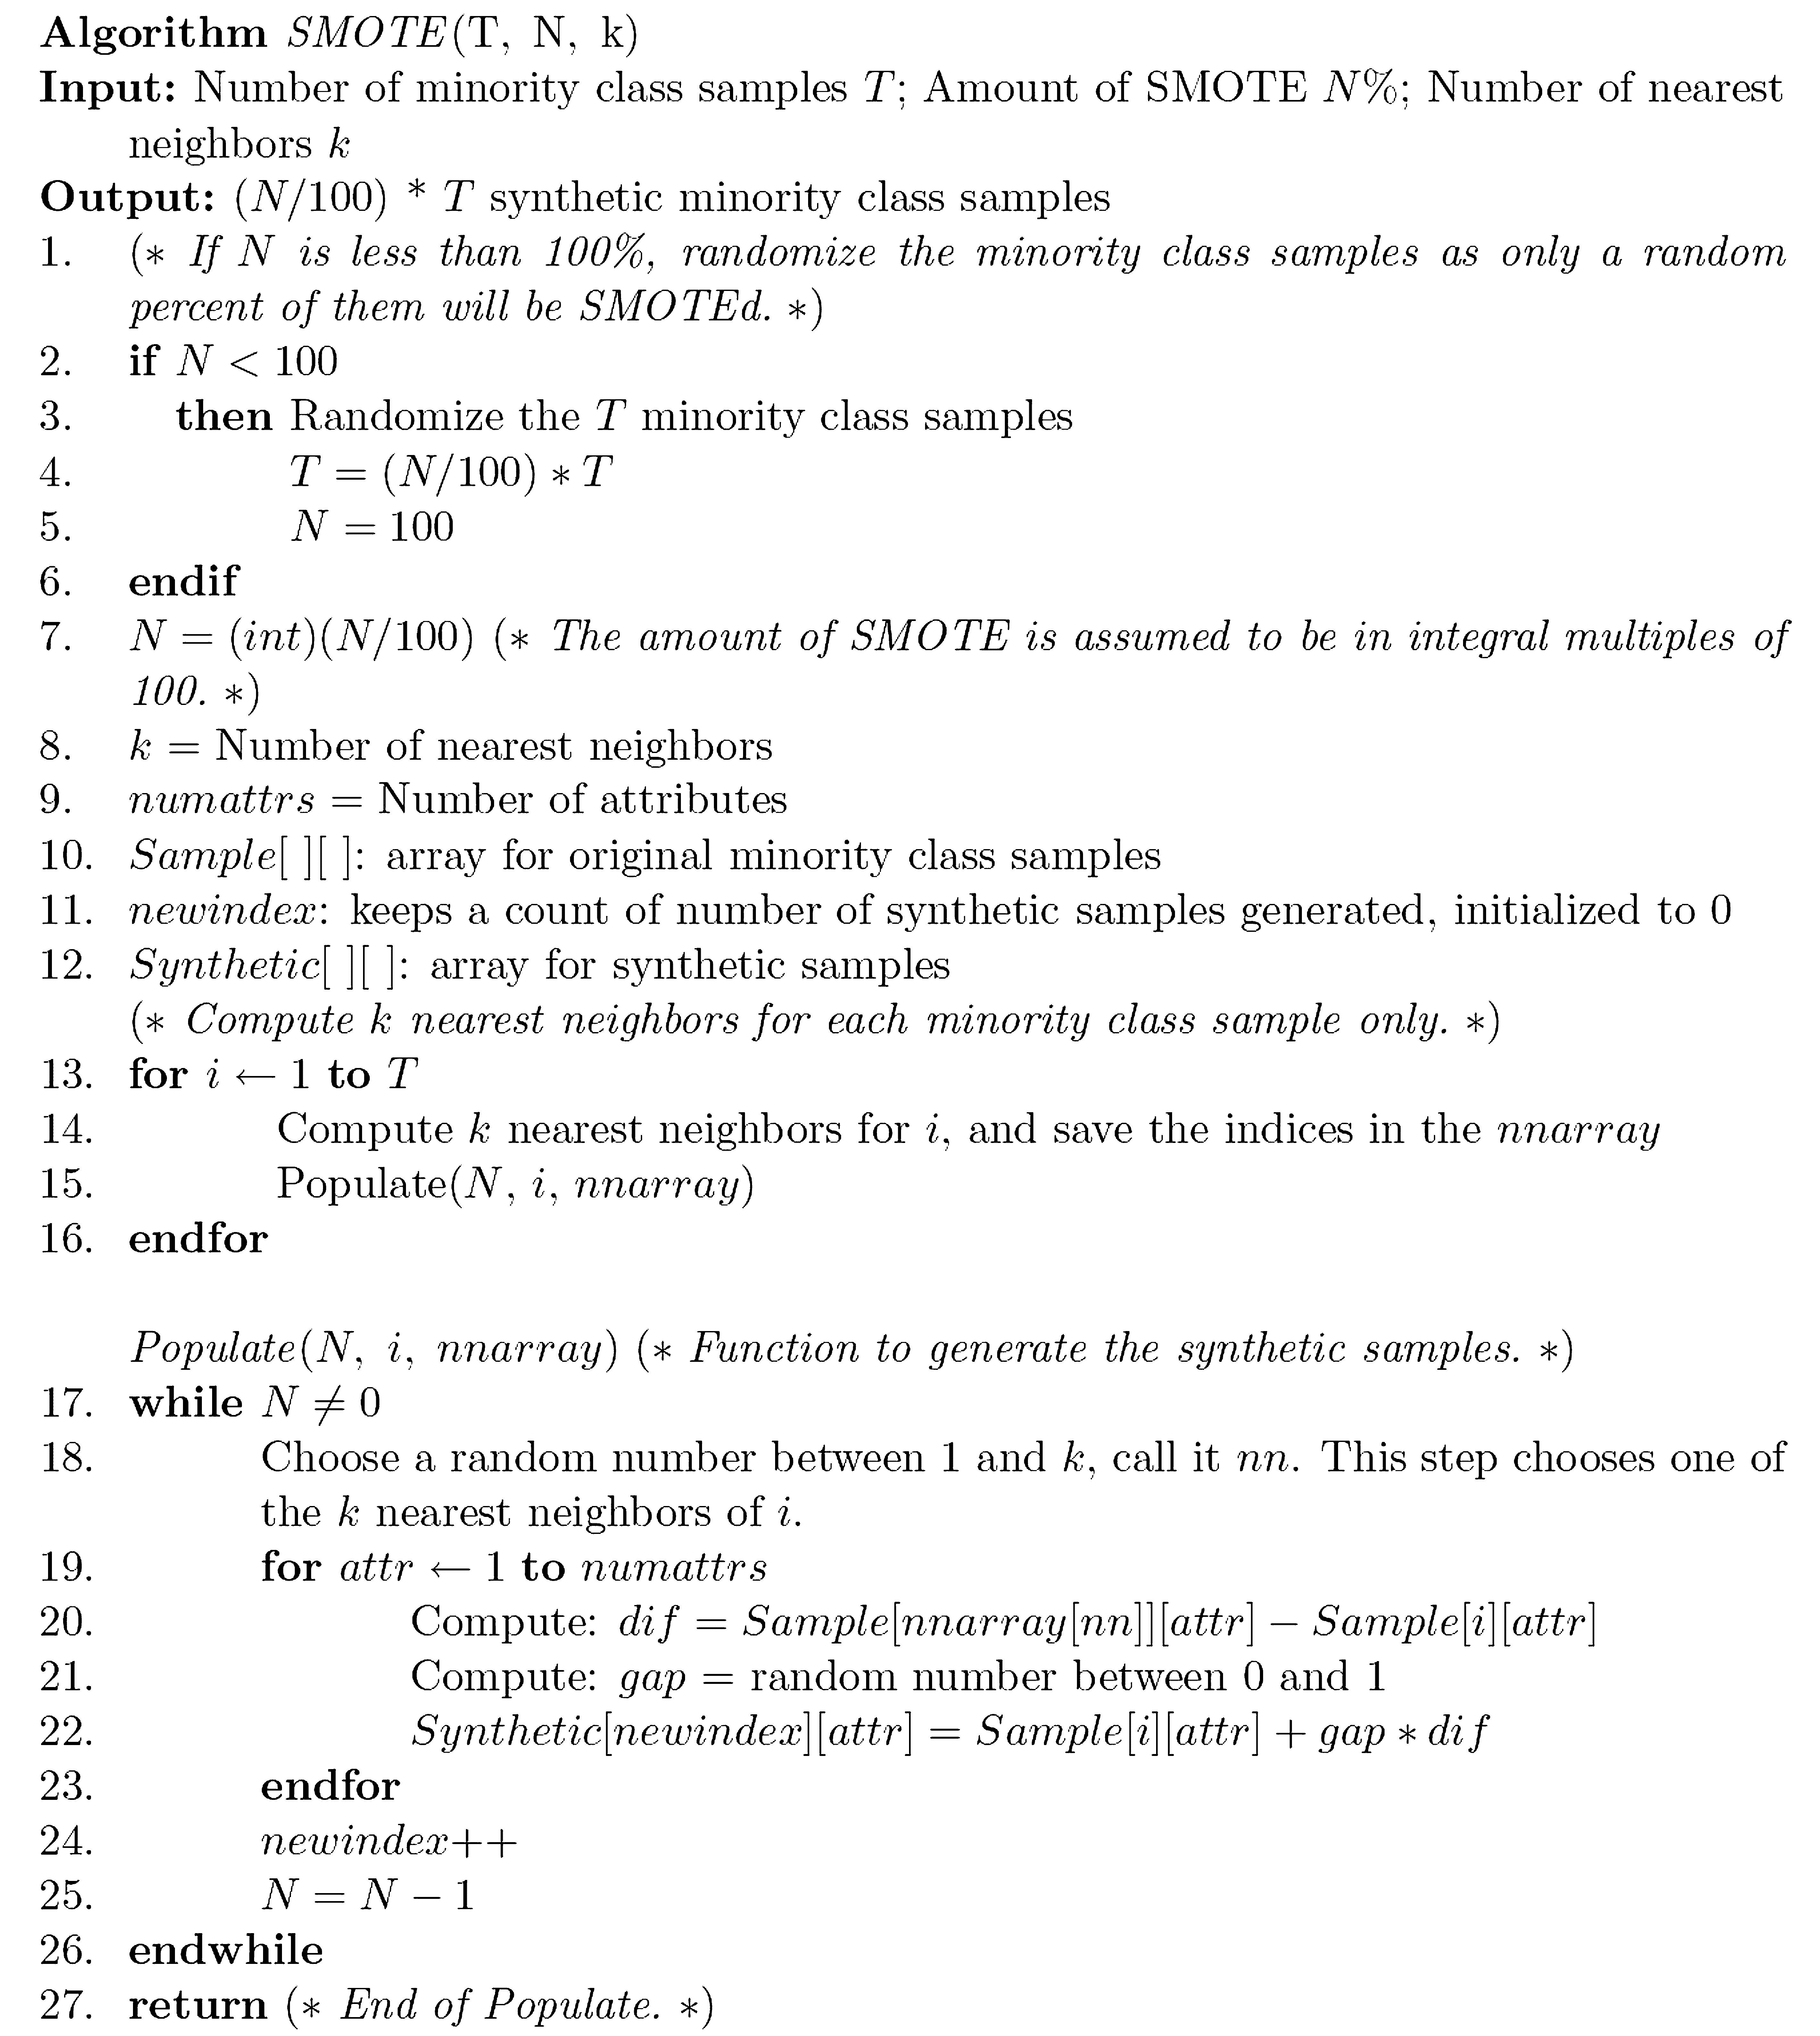
\includegraphics[width=\linewidth]{SMOTE_pseudocode.jpg}
  \caption{The Pseudocode for SMOTE. From \cite{smote}}
\end{figure}

\begin{figure}[!htbp]
  \renewcommand{\baselinestretch}{1.25}\begin{center}
    {\scriptsize
      \begin{tabular}{l@{~~~}l@{~~~}l@{~~~}l@{~~~}c@{~~~}l@{~~~}l@{~~~}}
        \hline
        \rowcolor{lightgray}
        Data & Symbol & Training & Testing & Training Samples& Defective &\% Defective \\\hline
        
        Ant & ant & 1.5, 1.6  &1.7 & 644&124&19.25\\
        
        Camel & cam & 1.2, 1.4 & 1.6 & 1480&361 & 24.39\\
        
        Ivy & ivy & 1.1, 1.4 & 2.0  & 352 & 79 & 22.44\\
        
        Jedit & jed & 4.1, 4.2 & 4.3 & 679 & 127 & 18.70\\
        
        Log4j & log & 1.0, 1.1 & 1.2 & 244 & 71 & 29.09\\
        
        Lucene & luc & 2.0, 2.2 & 2.4 & 442 & 235 & 53.16\\
        
        Poi & poi & 2.0, 2.5 & 3.0 & 699 & 285 & 40.77\\
        
        Synapse & syn & 1.0, 1.1 & 1.2 & 379 & 76 & 20.05\\
        
        Velocity & vel & 1.4, 1.5 & 1.6 & 410& 289 & 70.48\\
        
        Xalan & xal &2.5, 2.6 &2.7 & 1688 & 798 & 47.27\\\hline
      \end{tabular}}
    \end{center}
    \caption{Attributes of the defect data sets}\label{fig:attr}
  \end{figure}

\begin{algorithm}[htbp!]
  
  \scriptsize
  \begin{algorithmic}[1]
    \Require $\mathit{np} = 10$, $f=0.75$, $cr=0.3$, $\mathit{life} = 5$, $\mathit{Goal} \in \{\mathit{pd},f,...\}$
    \Ensure $S_{best}$
    
    ~\\
    \Function{DE}{$\mathit{np}$, $f$, $cr$, $\mathit{life}$, $\mathit{Goal}$}
    \State $Population  \gets $ $InitializePopulation$($\mathit{np}$)   
    \State $S_{best} \gets $$GetBestSolution$($Population $)
    \While{$\mathit{life} > 0$}
    \State $NewGeneration \gets \emptyset$
    \For{$i=0 \to \mathit{np}-1$}
    \State $S_i \gets$ Extrapolate($Population [i], Population , cr, f$)
    \If {Score($S_i$)$\ge$Score($Population [i]$)}
    \State $NewGeneration$.$append$($S_i$)
    \Else
    \State $NewGeneration$.$append$($Population [i]$)
    \EndIf
    \EndFor
    \State $Population  \gets NewGeneration$
    \If{$\neg$ $Improve$($Population $)}
    \State $life -=1$
    \EndIf
    \State $S_{best} \gets$ $GetBestSolution$($Population $)
    \EndWhile
    \State \Return $S_{best}$
    \EndFunction
    \Function{Score}{$Candidate$}
    \State set tuned parameters according to $Candidate$
    \State $model \gets$$TrainLearner()$
    \State $result \gets$$TestLearner$($model$)   
    \State \Return$\mathit{Goal}(result)$  
    \EndFunction
    \Function{Extrapolate}{$old, pop, cr, f$}
    \State $a, b, c\gets threeOthers(pop,old)$  
    \State $newf \gets \emptyset$
    \For{$i=0 \to \mathit{np}-1$}
    \If{$cr < random()$}
    \State $newf$.$append$($old[i]$)
    \Else
    \If{typeof($old[i]$) == bool}
    \State $newf$.$append$(not $old[i]$)
    \Else
    \State $newf$.$append$(trim($i$,($a[i] + f * (b[i] - c[i]$)))) 
    \EndIf
    \EndIf
    \EndFor
    \State \Return $newf$
    \EndFunction
  \end{algorithmic} 
  \caption{Pesudocode for DE with Early Termination}
  \label{alg:DE}
\end{algorithm}
\section{Experimental Setup}
\subsection{Data Sets}
\begin{figure*}[htbp!]
  \renewcommand{\baselinestretch}{1}\begin{center}
    {\scriptsize
      \begin{tabular}{c|l|p{4.7in}}
        amc & average method complexity & e.g. number of JAVA byte codes\\\hline
        avg\_cc & average McCabe & average McCabe's cyclomatic complexity seen
        in class\\\hline
        ca & afferent couplings & how many other classes use the specific
        class. \\\hline
        cam & cohesion amongst classes & summation of number of different
        types of method parameters in every method divided by a multiplication
        of number of different method parameter types in whole class and
        number of methods. \\\hline
        cbm &coupling between methods &  total number of new/redefined methods
        to which all the inherited methods are coupled\\\hline
        cbo & coupling between objects & increased when the methods of one
        class access services of another.\\\hline
        ce & efferent couplings & how many other classes is used by the
        specific class. \\\hline
        dam & data access & ratio of the number of private (protected)
        attributes to the total number of attributes\\\hline
        dit & depth of inheritance tree &\\\hline
        ic & inheritance coupling &  number of parent classes to which a given
        class is coupled (includes counts of methods and variables inherited)
        \\\hline
        lcom & lack of cohesion in methods &number of pairs of methods that do
        not share a reference to an instance variable.\\\hline
        locm3 & another lack of cohesion measure & if $m,a$ are  the number of
        $methods,attributes$
        in a class number and $\mu(a)$  is the number of methods accessing an
        attribute, 
        then
        $lcom3=((\frac{1}{a} \sum_j^a \mu(a_j)) - m)/ (1-m)$.
        \\\hline
        loc & lines of code &\\\hline
        max\_cc & maximum McCabe & maximum McCabe's cyclomatic complexity seen
        in class\\\hline
        mfa & functional abstraction & number of methods inherited by a class
        plus number of methods accessible by member methods of the
        class\\\hline
        moa &  aggregation &  count of the number of data declarations (class
        fields) whose types are user defined classes\\\hline
        noc &  number of children &\\\hline
        npm & number of public methods & \\\hline
        rfc & response for a class &number of  methods invoked in response to
        a message to the object.\\\hline
        wmc & weighted methods per class &\\\hline
        \rowcolor{lightgray}
        defect & defect & Boolean: where defects found in post-release bug-tracking systems.
      \end{tabular}
    }
  \end{center}
  \caption{OO measures used in our defect data sets.  Last line is
    the dependent attribute (whether a defect is reported to  a
    post-release bug-tracking system).}\label{fig:ck}
\end{figure*}

\section{Experimental Results}
\begin{table*}[htbp!]
  \renewcommand{\baselinestretch}{1.25}
  \begin{subtable}{0.5\linewidth}
    
    {\tiny \begin{tabulary}{\linewidth}{|J|J|J|J|J|}
        \hline
        \textbf{Rank} & \textbf{Treatment} & \textbf{Med} & \textbf{IQR} & \\\hline
        1 &   RF &    41.0  &  3.0 & \quart{0}{7}{2}{-102} \\
        \hline  2 &   CART &    44.0  &  3.0 & \quart{10}{8}{10}{-102} \\
        \hline  3 & CART (SMOTE) &    70.0  &  2.0 & \quart{76}{5}{78}{-102} \\
        \hline  4 & RF (SMOTE) &    78.0  &  1.0 & \quart{97}{2}{99}{-102} \\[0.1cm]
        \hline \end{tabulary}} \caption{ant} \label{ant}
    
  \end{subtable}
  \begin{subtable}{0.5\linewidth}
    {\tiny \begin{tabulary}{\linewidth}{|J|J|J|J|J|}
        \hline
        \textbf{Rank} & \textbf{Treatment} & \textbf{Med} & \textbf{IQR} & \\\hline
        1 & RF &    39.0  &  1.0 & \quart{0}{4}{0}{-172} \\
        \hline  2 & CART &    43.0  &  2.0 & \quart{9}{9}{18}{-172} \\
        \hline  3 & CART (SMOTE) &    56.0  &  2.0 & \quart{72}{9}{77}{-172} \\
        \hline  4 & RF (SMOTE) &    60.0  &  2.0 & \quart{90}{9}{95}{-172} \\
        \hline \end{tabulary}}\caption{Camel} \label{Camel}
    
  \end{subtable}\\[0.2cm]
  
  \begin{subtable}{0.5\linewidth}
    {\tiny \begin{tabulary}{\linewidth}{|J|J|J|J|J|}
        \hline
        \textbf{Rank} & \textbf{Treatment} & \textbf{Med} & \textbf{IQR} & \\\hline
        1 & RF (SMOTE) &    0.0  &  0.0 & \quart{0}{0}{0}{1} \\
        1 & CART (SMOTE) &    15.0  &  15.0 & \quart{0}{26}{26}{1} \\
        \hline  2 &   RF &    50.0  &  1.0 & \quart{85}{2}{87}{1} \\
        \hline  3 &   CART &    56.0  &  1.0 & \quart{98}{1}{98}{1} \\
        \hline \end{tabulary}}\caption{Ivy} \label{Camel}
    
  \end{subtable}
  \begin{subtable}{0.5\linewidth}
    {\tiny \begin{tabulary}{\linewidth}{|J|J|J|J|J|}
        \hline
        \textbf{Rank} & \textbf{Treatment} & \textbf{Med} & \textbf{IQR} & \\\hline
        1 & RF &    0.0  &  0.0 & \quart{0}{0}{0}{1} \\
        1 & CART (SMOTE) &    84.0  &  1.0 & \quart{89}{1}{90}{1} \\
        1 & RF (SMOTE) &    88.0  &  1.0 & \quart{93}{1}{94}{1} \\
        1 & CART &    93.0  &  0.0 & \quart{99}{0}{99}{1} \\
        \hline \end{tabulary}}\caption{Jedit} \label{Camel}
    
  \end{subtable}\\[0.2cm]
  
  \begin{subtable}{0.5\linewidth}
    {\tiny \begin{tabulary}{\linewidth}{|J|J|J|J|J|}
        \hline
        \textbf{Rank} & \textbf{Treatment} & \textbf{Med} & \textbf{IQR} & \\\hline
        1 &   CART &    36.0  &  3.0 & \quart{0}{14}{0}{-166} \\
        1 &   RF &    40.0  &  4.0 & \quart{4}{19}{19}{-166} \\
        \hline  2 & RF (SMOTE) &    53.0  &  6.0 & \quart{71}{28}{80}{-166} \\
        2 & CART (SMOTE) &    54.0  &  4.0 & \quart{76}{19}{85}{-166} \\
        \hline \end{tabulary}}\caption{POI} \label{Camel}
    
  \end{subtable}
  \begin{subtable}{0.5\linewidth}
    {\tiny \begin{tabulary}{\linewidth}{|J|J|J|J|J|}
        \hline
        \textbf{Rank} & \textbf{Treatment} & \textbf{Med} & \textbf{IQR} & \\\hline
        1 & RF (SMOTE) &    2.0  &  2.0 & \quart{0}{4}{2}{0} \\
        \hline  2 & CART (SMOTE) &    14.0  &  5.0 & \quart{31}{12}{31}{0} \\
        \hline  3 & RF &    22.0  &  2.0 & \quart{48}{5}{51}{0} \\
        \hline  4 & CART &    41.0  &  2.0 & \quart{95}{4}{97}{0} \\
        \hline \end{tabulary}}\caption{Log4j} \label{Camel}
    
  \end{subtable}\\[0.2cm]
  
  \begin{subtable}{0.5\linewidth}
    {\tiny \begin{tabulary}{\linewidth}{|J|J|J|J|J|}
        \hline
        \textbf{Rank} & \textbf{Treatment} & \textbf{Med} & \textbf{IQR} & \\\hline
        1 & CART &    47.0  &  1.0 & \quart{0}{9}{0}{-418} \\
        \hline  2 & RF &    51.0  &  1.0 & \quart{36}{9}{36}{-418} \\
        2 & CART (SMOTE) &    50.0  &  4.0 & \quart{27}{36}{27}{-418} \\
        \hline  3 & RF (SMOTE) &    56.0  &  3.0 & \quart{72}{27}{81}{-418} \\
        \hline \end{tabulary}}\caption{Lucene} \label{Camel}
    
  \end{subtable}
  \begin{subtable}{0.5\linewidth}
    {\tiny \begin{tabulary}{\linewidth}{|J|J|J|J|J|}
        \hline
        \textbf{Rank} & \textbf{Treatment} & \textbf{Med} & \textbf{IQR} & \\\hline
        1 & RF &    51.0  &  0.0 & \quart{49}{0}{49}{-449} \\
        1 & CART &    53.0  &  0.0 & \quart{69}{0}{69}{-449} \\
        1 & CART (SMOTE) &    56.0  &  10.0 & \quart{0}{99}{99}{-449} \\
        1 & RF (SMOTE) &    56.0  &  1.0 & \quart{89}{10}{99}{-449} \\
        \hline \end{tabulary}}\caption{PBeans} \label{Camel}
    
  \end{subtable}\\[0.2cm]
  
  
  \begin{subtable}{0.5\linewidth}
    {\tiny \begin{tabulary}{\linewidth}{|J|J|J|J|J|}
        \hline
        \textbf{Rank} & \textbf{Treatment} & \textbf{Med} & \textbf{IQR} & \\\hline
        1 & CART (SMOTE) &    63.0  &  1.0 & \quart{0}{9}{9}{-609} \\
        \hline  2 & RF (SMOTE) &    68.0  &  2.0 & \quart{39}{20}{59}{-609} \\
        \hline  3 & CART &    70.0  &  2.0 & \quart{59}{20}{79}{-609} \\
        3 & RF &    70.0  &  2.0 & \quart{79}{20}{79}{-609} \\
        \hline \end{tabulary}}\caption{Velocity} \label{Camel}
    
  \end{subtable}
  \begin{subtable}{0.5\linewidth}
    {\tiny \begin{tabulary}{\linewidth}{|J|J|J|J|J|}
        \hline
        \textbf{Rank} & \textbf{Treatment} & \textbf{Med} & \textbf{IQR} & \\\hline
        1 & RF &    24.0  &  1.0 & \quart{0}{2}{0}{-58} \\
        \hline  2 & CART &    52.0  &  18.0 & \quart{53}{46}{71}{-58} \\
        2 & CART (SMOTE) &    59.0  &  2.0 & \quart{84}{5}{89}{-58} \\
        2 & RF (SMOTE) &    60.0  &  1.0 & \quart{92}{2}{92}{-58} \\
        \hline \end{tabulary}}\caption{Xalan} \label{Camel}
    
  \end{subtable}
  \caption{Performance scores (g values) for the data sets.}
\end{table*}
\subsection{SMOTE\textit{ing} improves Prediction Accuracy}
\subsection{Tuning Also improves Prediction Accuracy (?)}
\subsection{SMOTE\textit{ing}+Tuning improves Prediction Accuracy (?)}
\section{Conclusions}
\bibliographystyle{IEEEtran}
\bibliography{Ref}
\end{document}